When other academic studies dealing with the measurement of maintainability of software systems were reviewed, it was seen that many studies use quantitative methods. When the quantitative evaluations made in these studies are examined, it is seen that Android applications use several object-oriented software metrics while evaluating maintainability. Details of these studies were shared earlier in section \ref{section:3.2}. Although it cannot be claimed that such quantitative measurements are inaccurate, it would not be wrong to say that these measures are inadequate at times. It is essential to make qualitative evaluations and quantitative evaluations to increase the efficiency of the evaluations. In this way, it may be possible to measure developers' experiences and their effects on maintainability. For these reasons, an Android developer survey and interviews were conducted within this study's scope. This section covers these qualitative methods.

\subsubsection{Android Developer Survey}
\label{section:4.1.1}
The survey accepted answers between April 2020 and March 2021 and reached 164 participants in total.
\begin{figure}[ht!]
    \centering
    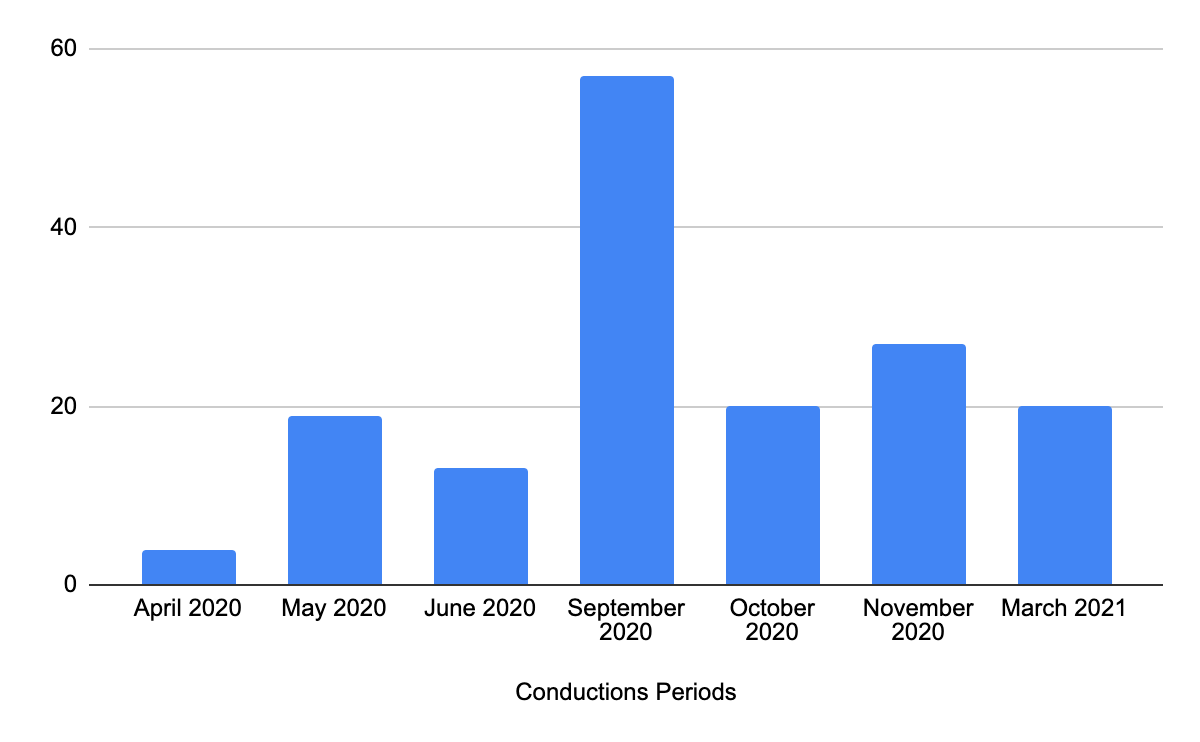
\includegraphics[scale=0.3]{figures/survey_conduction_period.png}
    \caption{Conduction period results}
    \label{fig:conduction_period}
\end{figure}

As shown in Fig. \ref{fig:conduction_period}, participation in the survey took place only during specific periods of this one-year term. Although the questionnaire accepted answers for a year-long, it was boosted in different periods,  as shown in the histogram above. It would be logical to consider this situation while examining the response numbers.

\subsubsection{Interviews with Team Members}
\label{section:4.1.2}
The second step of the qualitative evaluations carried out within this study’s scope is the interviews conducted with Mooncascade's Android team members.  The interview questions are designed to qualitatively evaluate the techniques and technologies used by Mooncascade's Android team in terms of maintainability. Also, the interviews aim to determine the importance of maintainability from the case company's point of view.  Thus, proving or disproving the study's claim that maintainability is a key concept to overcome the issues mentioned in the problem statement section would be possible. Eight questions were determined for these purposes. Below are listed the questions asked to each member of Mooncascade's Android team during these interviews:
\begin{itemize}
    \item How many years of experience do you have as an Android developer? Please specify the years in Mooncascade and other companies.
    \item How many different Android projects have you completed in Mooncascade, and how many different domains did those projects belong to?
    \item What is your understanding of maintainability in the context of software engineering?
    \item As an employee of a software development company that provides services to the different domains, what makes maintainability more essential for you?
    \item What is the importance of maintainability when developing Android applications?
    \item What is the most critical aspect for maintainability when developing Android applications (e.g. architecture, libraries, programming language, etc.)?
    \item How do you think the current technology stack of the team impacts Android applications’ maintainability? Please specify for each item below:
    \begin{itemize}
        \item Programming Languages(Kotlin/Java)
        \item Software Engineering principles (SOLID/Clean Code)
        \item Architecture (MVVM/Clean)
        \item Libraries (RxJava, Dagger 2, Apollo/Retrofit)
        \item Android Architecture Components (ViewModel, LiveData, Room, etc.)
    \end{itemize}
    \item What could be improved in our current tech stack and the principles we apply to improve the Android applications’ maintainability?
\end{itemize}

Three main criteria were taken into consideration while preparing these questions. First of all, questions were chosen to get to know about the participants' background and experience. Later, some questions were designed to learn participants' understanding of maintainability in software engineering. Lastly, questions were drafted to learn about participants' thoughts about the impact of technologies and principles used by Mooncascade on maintainability. The interview was conducted privately with each team member.  It is aimed that the data gathered through these interviews will increase the accuracy and validity of evaluations.
